% MDPI AI submission package adapted from the official MDPI template.

\documentclass[ai,article,submit,pdftex,oneauthor]{Definitions/mdpi}

\firstpage{1}
\makeatletter
\setcounter{page}{\@firstpage}
\makeatother
\pubvolume{1}
\issuenum{1}
\articlenumber{0}
\pubyear{2026}
\copyrightyear{2026}
\datereceived{}
\daterevised{}
\dateaccepted{}
\datepublished{}

\setlength{\headheight}{20pt}

\externalbibliography{yes}

\Title{Attention Structural Change During CLIP Fine-Tuning: A Comparative Study of Full Fine-Tuning, LoRA, and Regularization}

\Author{Ruize Xia $^{1}$\orcidA{}}
\AuthorNames{Ruize Xia}
\newcommand{\orcidauthorA}{0009-0000-0501-0943} 

\address{%
$^{1}$ \quad Nanjing Foreign Language School, Nanjing, Jiangsu, China; xiaruize0911@gmail.com}

\corres{Correspondence: xiaruize0911@gmail.com}

\abstract{Fine-tuning contrastive vision--language models such as CLIP is an essential step for downstream task specialization, yet the associated changes in the internal attention geometry remain insufficiently characterized. This study investigates the CLIP ViT-B/32 visual encoder across 21 experimental configurations on EuroSAT and Oxford-IIIT Pets, comparing full fine-tuning, low-rank adaptation (LoRA), and explicit attention-based regularization. We employ a multi-faceted metric suite—including CLS-to-patch attention entropy, effective receptive field (ERF), Gini concentration, and head diversity—complemented by attention rollout, CKA representational analysis, and subset-sensitivity tests. Our results demonstrate that full fine-tuning generally induces a contraction of attention support, whereas LoRA configurations maintain or even broaden the spatial distribution relative to the pretrained baseline. Statistical analysis via exact permutation tests identifies the learning rate as a critical determinant of these structural shifts. Furthermore, zero-shot reevaluation confirms that while LoRA incurs minor transfer degradation, it remains significantly more conservative than full fine-tuning. These findings provide a new structural lens for understanding the dynamics of transformer adaptation and suggest that structural preservation is a key mechanism for maintaining the generalizability of foundation models.}

\keyword{CLIP; vision--language models; foundation models; transformer adaptation; LoRA; attention analysis; structural collapse; computer vision}

\begin{document}

\section{Introduction}
Contrastive vision--language pretraining has established CLIP as a foundational architecture for cross-modal retrieval and zero-shot visual recognition~\cite{radford2021learning,shao2023vlm}. Despite its impressive zero-shot capabilities, practical deployment often requires downstream adaptation to achieve competitive performance on specialized domains. However, recent evidence suggests that such fine-tuning can distort the well-calibrated pretrained feature space, leading to significant performance drops in out-of-distribution (OOD) scenarios~\cite{kumar2022finetuning,wortsman2022robust}. While the functional impact of this distortion is well-documented, the internal structural evolution of the self-attention mechanism during adaptation—specifically for CLIP—remains a subject of active research.

Self-attention is the central mechanism for long-range dependency modeling in Vision Transformers (ViT)~\cite{vaswani2017attention,dosovitskiy2021image}. Prior work has shown that pretrained ViTs develop specialized attention patterns, such as global context aggregation and local feature extraction, which are critical for robust representation learning~\cite{raghu2021vision,caron2021emerging}. Understanding whether these patterns are preserved or overwritten during fine-tuning is vital for developing safer and more interpretable adaptation strategies. In this paper, we focus on the concept of \emph{attention structural change}, exploring how different optimization regimes reshape the spatial allocation of attention mass.

We adopt a descriptive framework for attention analysis, treating measurements as indicators of model state rather than direct causal drivers of inference~\cite{wiegreffe2019attention,chefer2021transformer}. This distinction is necessary because the mapping from attention weights to model decisions is complex and often non-linear~\cite{jain2019attention}. By focusing on structural descriptors—such as entropy, Gini concentration, and effective receptive field—we quantify the "plasticity" of the CLIP visual encoder under different constraints.

The study addresses four primary research questions: (i) the extent to which full fine-tuning alters the spatial concentration of attention; (ii) how parameter-efficient methods like LoRA differ from full fine-tuning in their structural impact; (iii) the role of hyperparameter selection, particularly the learning rate, in driving these changes; and (iv) the feasibility of mitigating structural drift through explicit regularization. Our contributions include:
\begin{itemize}
    \item an empirical characterization of structural evolution in CLIP under varying adaptation regimes;
    \item a comprehensive evaluation of LoRA's structural conservatism and its implications for transfer learning;
    \item the identification of learning rate as a dominant control variable for attention concentration; and
    \item a systematic evaluation of various attention-based regularization techniques.
\end{itemize}

\section{Related Work}
The landscape of large-scale vision--language pretraining and downstream adaptation has evolved rapidly, centered on the dual challenges of performance and robustness. Therefore, we review the relevant literature across four interconnected domains: Vision Transformers (ViT), contrastive vision--language models (CLIP), fine-tuning dynamics and feature distortion, and parameter-efficient fine-tuning methods such as LoRA.

\subsection{Vision Transformers (ViT)}
The Vision Transformer (ViT) architecture~\cite{dosovitskiy2021image} shifted the computer vision paradigm by applying the self-attention mechanism~\cite{vaswani2017attention} to image patches. Unlike Convolutional Neural Networks (CNNs), ViTs lack inductive biases like translation invariance, relying instead on massive datasets to learn spatial hierarchies. Studies on ViT internal representations reveal that they develop distinct "attention heads" for global context and local feature extraction~\cite{raghu2021vision}, and exhibit emergent properties such as object segmentation when trained with self-supervision~\cite{caron2021emerging}.

\subsection{Contrastive Vision--Language Models (CLIP)}
CLIP (Contrastive Language--Image Pretraining)~\cite{radford2021learning} scales ViT-based visual encoders by aligning them with text encoders using a contrastive loss on millions of image-text pairs. This alignment enables zero-shot classification across diverse datasets. However, CLIP's general-purpose features are often suboptimal for specialized domains, necessitating downstream fine-tuning. Benchmarking studies like \cite{shao2023vlm} highlight that while CLIP is a robust foundation, its performance varies significantly across task-specific distributions.

\subsection{Fine-Tuning and Feature Distortion}
Standard full fine-tuning (Full FT) updates all model parameters to maximize in-domain accuracy. While effective, this process can lead to "feature distortion," where the well-distributed pretrained embeddings collapse into narrow, task-specific manifolds~\cite{kumar2022finetuning}. Wortsman et al.~\cite{wortsman2022robust} observed that fine-tuning often degrades the model's out-of-distribution (OOD) robustness, prompting the development of weight-ensembling and constrained optimization techniques to preserve the pretrained knowledge.

\subsection{Low-Rank Adaptation (LoRA)}
To mitigate the computational cost and "forgetting" issues of full fine-tuning, parameter-efficient fine-tuning (PEFT) methods have gained prominence. LoRA (Low-Rank Adaptation)~\cite{hu2022lora} freezes the pretrained weights and injects trainable low-rank matrices into the attention projections. This significantly reduces the degrees of freedom during optimization. While initially developed for Large Language Models (LLMs), LoRA has become a standard for adapting vision models, though its impact on the internal attention structure of multimodal encoders like CLIP remains less explored.

\subsection{Attention Analysis and Interpretability}
The interpretability of self-attention distributions is a subject of ongoing debate. While attention maps are often used to identify "important" regions of an image, Jain and Wallace~\cite{jain2019attention} argued that they do not always provide a faithful explanation of model decisions. Conversely, Wiegreffe and Pinter~\cite{wiegreffe2019attention} and Chefer et al.~\cite{chefer2021transformer} emphasized that attention provides a valuable structural roadmap of information flow, especially when aggregated via methods like attention rollout~\cite{abnar2020quantifying}. We follow this structural perspective to measure the geometric shifts occurring during CLIP adaptation.

\section{Materials and Methods}
\subsection{Problem Formulation}
Let $f_0$ represent the weights of a pretrained CLIP vision encoder. During adaptation, we minimize a cross-entropy loss $\mathcal{L}_{\mathrm{task}}$ to obtain updated weights $\theta$. We monitor the CLS-to-patch attention distributions $A$ across all layers $\ell \in \{1, \dots, 12\}$. Since the CLS token serves as the primary conduit for global feature synthesis in the CLIP ViT-B/32 architecture, its attention profile provides a direct measure of how information is sampled from the spatial tokens.

\subsection{Structural Metrics}
We define four primary metrics to quantify the spatial geometry of the CLS-to-patch attention vectors $a \in \mathbb{R}^{49}$.

\subsubsection{Attention Entropy}
We quantify the uncertainty or "spread" of the distribution using Shannon entropy:
\begin{equation}
H(a) = -\sum_{j=1}^{49} a_j \ln a_j.
\end{equation}
Consistent with standard practice in transformer analysis, we report entropy in nats. A decrease in entropy indicates a more concentrated attention focus.

\subsubsection{Effective Receptive Field (ERF@0.95)}
To measure the spatial fraction of the image required to account for the majority of the attention mass, we define:
\begin{equation}
\mathrm{ERF}_{0.95}(a) = \frac{1}{49} \min\Big\{k : \sum_{j=1}^{k} a_{(j)} \geq 0.95\Big\},
\end{equation}
where $a_{(j)}$ are the sorted attention weights. This metric is particularly useful for identifying models that rely on a very small subset of tokens.

\subsubsection{Gini Concentration}
The Gini coefficient measures the inequality within the attention distribution. A Gini value of 0 indicates a perfectly uniform distribution, while a value approaching 1 indicates extreme sparsity where nearly all mass is allocated to a single token.

\subsubsection{Head Diversity}
Transformer layers typically employ multiple heads to capture diverse feature relations~\cite{vaswani2017attention}. We define head diversity as $1 - \bar{\rho}$, where $\bar{\rho}$ is the mean pairwise cosine similarity between the CLS-to-patch attention maps of all heads within a layer. Lower diversity suggests a collapse of head-wise specialization.

\subsection{Additional Validation Metrics}
To ensure the robustness of our findings, we incorporate auxiliary analyses. Attention rollout~\cite{abnar2020quantifying} provides a multi-layer view of routing. Layerwise centered kernel alignment (CKA) is used to measure the similarity between pretrained and fine-tuned feature representations. Subset-sensitivity analysis serves as a control for dataset-specific artifacts, ensuring that the observed structural shifts are representative of the model's behavior rather than noise in a specific evaluation batch.

\subsection{Experimental Setup}
Our experiments utilize the \texttt{openai/clip-vit-base-patch32} model. We evaluate adaptation on EuroSAT~\cite{helber2019eurosat} (for remote sensing) and Oxford-IIIT Pets~\cite{parkhi2012cats} (for fine-grained classification). These datasets represent distinct visual domains, allowing us to assess the consistency of structural changes.

For the optimization, we use AdamW~\cite{loshchilov2019decoupled} with its standard implementation~\cite{kingma2015adam} and a cosine-decay schedule. In full fine-tuning (Full FT), all vision encoder parameters are updated. In LoRA, we insert low-rank adapters into the query and value projections (\texttt{q\_proj}, \texttt{v\_proj}) with rank $r=8$ and scaling $\alpha=16$. Experimental runs were standardized using NVIDIA A40 hardware to ensure reproducibility.


\subsection{Statistical Analysis}
Because per-layer measurements within a single model are not independent, per-layer $t$-tests are treated as exploratory rather than confirmatory. For the five-point learning-rate analysis, approximate small-sample $p$-values are therefore replaced with exact permutation tests. For the family of regularizer comparisons, Holm-Bonferroni-adjusted $p$-values are reported. The available evidence is nonetheless limited by the absence of multi-seed replications for the main training configurations.

\section{Results}
\subsection{Overall Comparison of Adaptation Regimes}
Table~\ref{tab:main-results} summarizes the central comparisons. Full fine-tuning reaches the highest EuroSAT validation accuracy (99.30\%) but slightly reduces average attention entropy ($-0.14\%$) and ERF ($-1.73\%$) relative to the pretrained baseline. On Pets, full fine-tuning produces a larger entropy decrease ($-1.82\%$), a larger ERF contraction ($-4.23\%$), and a substantial Gini increase ($+10.54\%$), indicating stronger concentration. By contrast, the EuroSAT LoRA configurations consistently increase entropy and reduce Gini relative to the baseline while keeping task accuracy above 98.6\%.

\begin{table*}[t]
\centering
\caption{Main experiment results. Positive $\Delta$Entropy and $\Delta$ERF indicate broader attention support relative to the corresponding pretrained baseline; positive $\Delta$Gini indicates more concentrated attention.}
\label{tab:main-results}
\small
\resizebox{\textwidth}{!}{%
\begin{tabular}{llrrrrrrr}
\toprule
Method & Dataset & Task Acc. (\%) & $\Delta$Entropy (\%) & $\Delta$ERF (\%) & $\Delta$Gini (\%) & $\Delta$HeadDiv (\%) & CIFAR-100 ZS (\%) & Flowers102 ZS (\%) \\
\midrule
Full FT & EuroSAT & 99.30 & -0.14 & -1.73 & -3.54 & -0.62 & 12.71 & 1.37 \\
Full FT & Oxford-IIIT Pets & 90.79 & -1.82 & -4.23 & +10.54 & -35.91 & 5.89 & 0.88 \\
LoRA r=4 & EuroSAT & 98.67 & +0.98 & +1.09 & -9.94 & +3.86 & 60.22 & 0.20 \\
LoRA r=8 & EuroSAT & 98.96 & +0.58 & +0.37 & -6.48 & +7.17 & 60.22 & 0.20 \\
LoRA r=16 & EuroSAT & 98.93 & +0.44 & +0.03 & -5.43 & +5.14 & 60.22 & 0.20 \\
LoRA r=8 & Oxford-IIIT Pets & 92.07 & -0.73 & -2.64 & +3.20 & -15.00 & --- & --- \\
\bottomrule
\end{tabular}
}
\end{table*}


Figure~\ref{fig:baseline-structure} shows that the pretrained model already exhibits heterogeneous attention structure across depth, so the appropriate question is not whether fine-tuning creates structure from nothing, but whether it pushes that structure toward greater concentration. Figure~\ref{fig:ft-vs-lora} then shows that full fine-tuning and LoRA trace visibly different trajectories in entropy, ERF, Gini, and head diversity.

\begin{figure}[H]
\centering
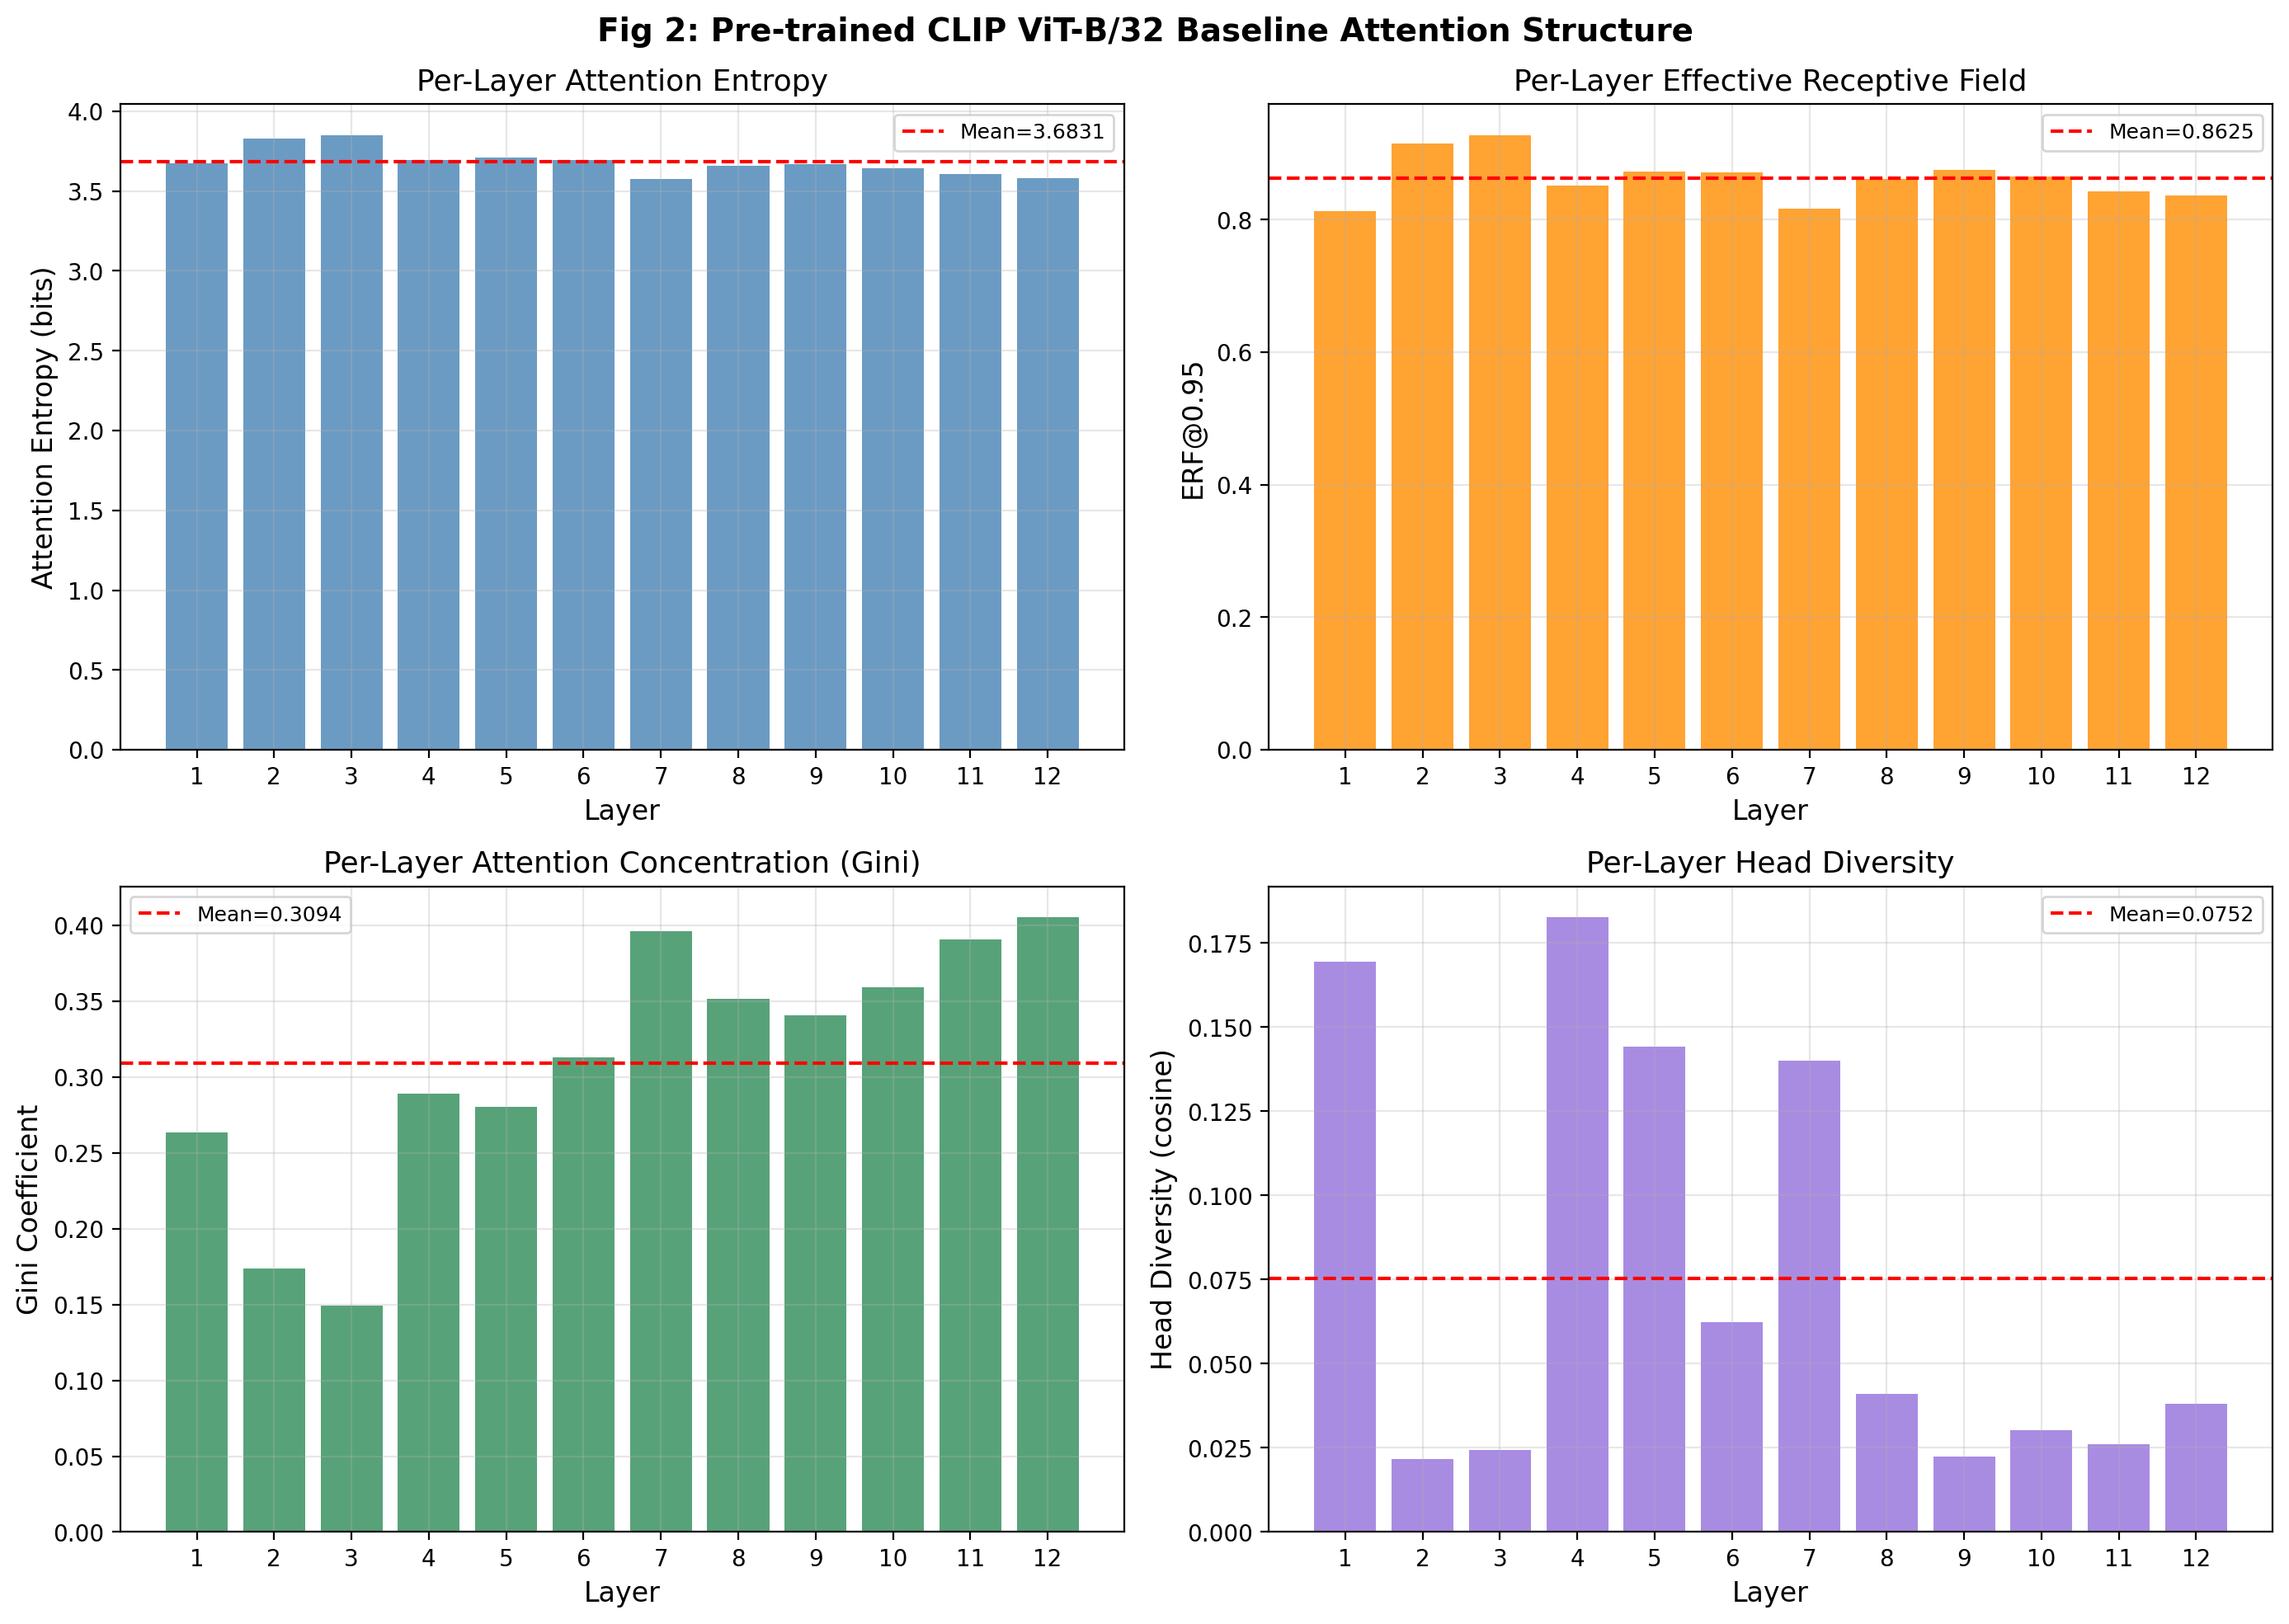
\includegraphics[width=\textwidth]{figures/fig2_baseline_structure.png}
\caption{Baseline attention structure of pretrained CLIP ViT-B/32 across layers. The model is already depth-heterogeneous before any downstream adaptation.}\label{fig:baseline-structure}
\end{figure}

\begin{figure}[H]
\centering
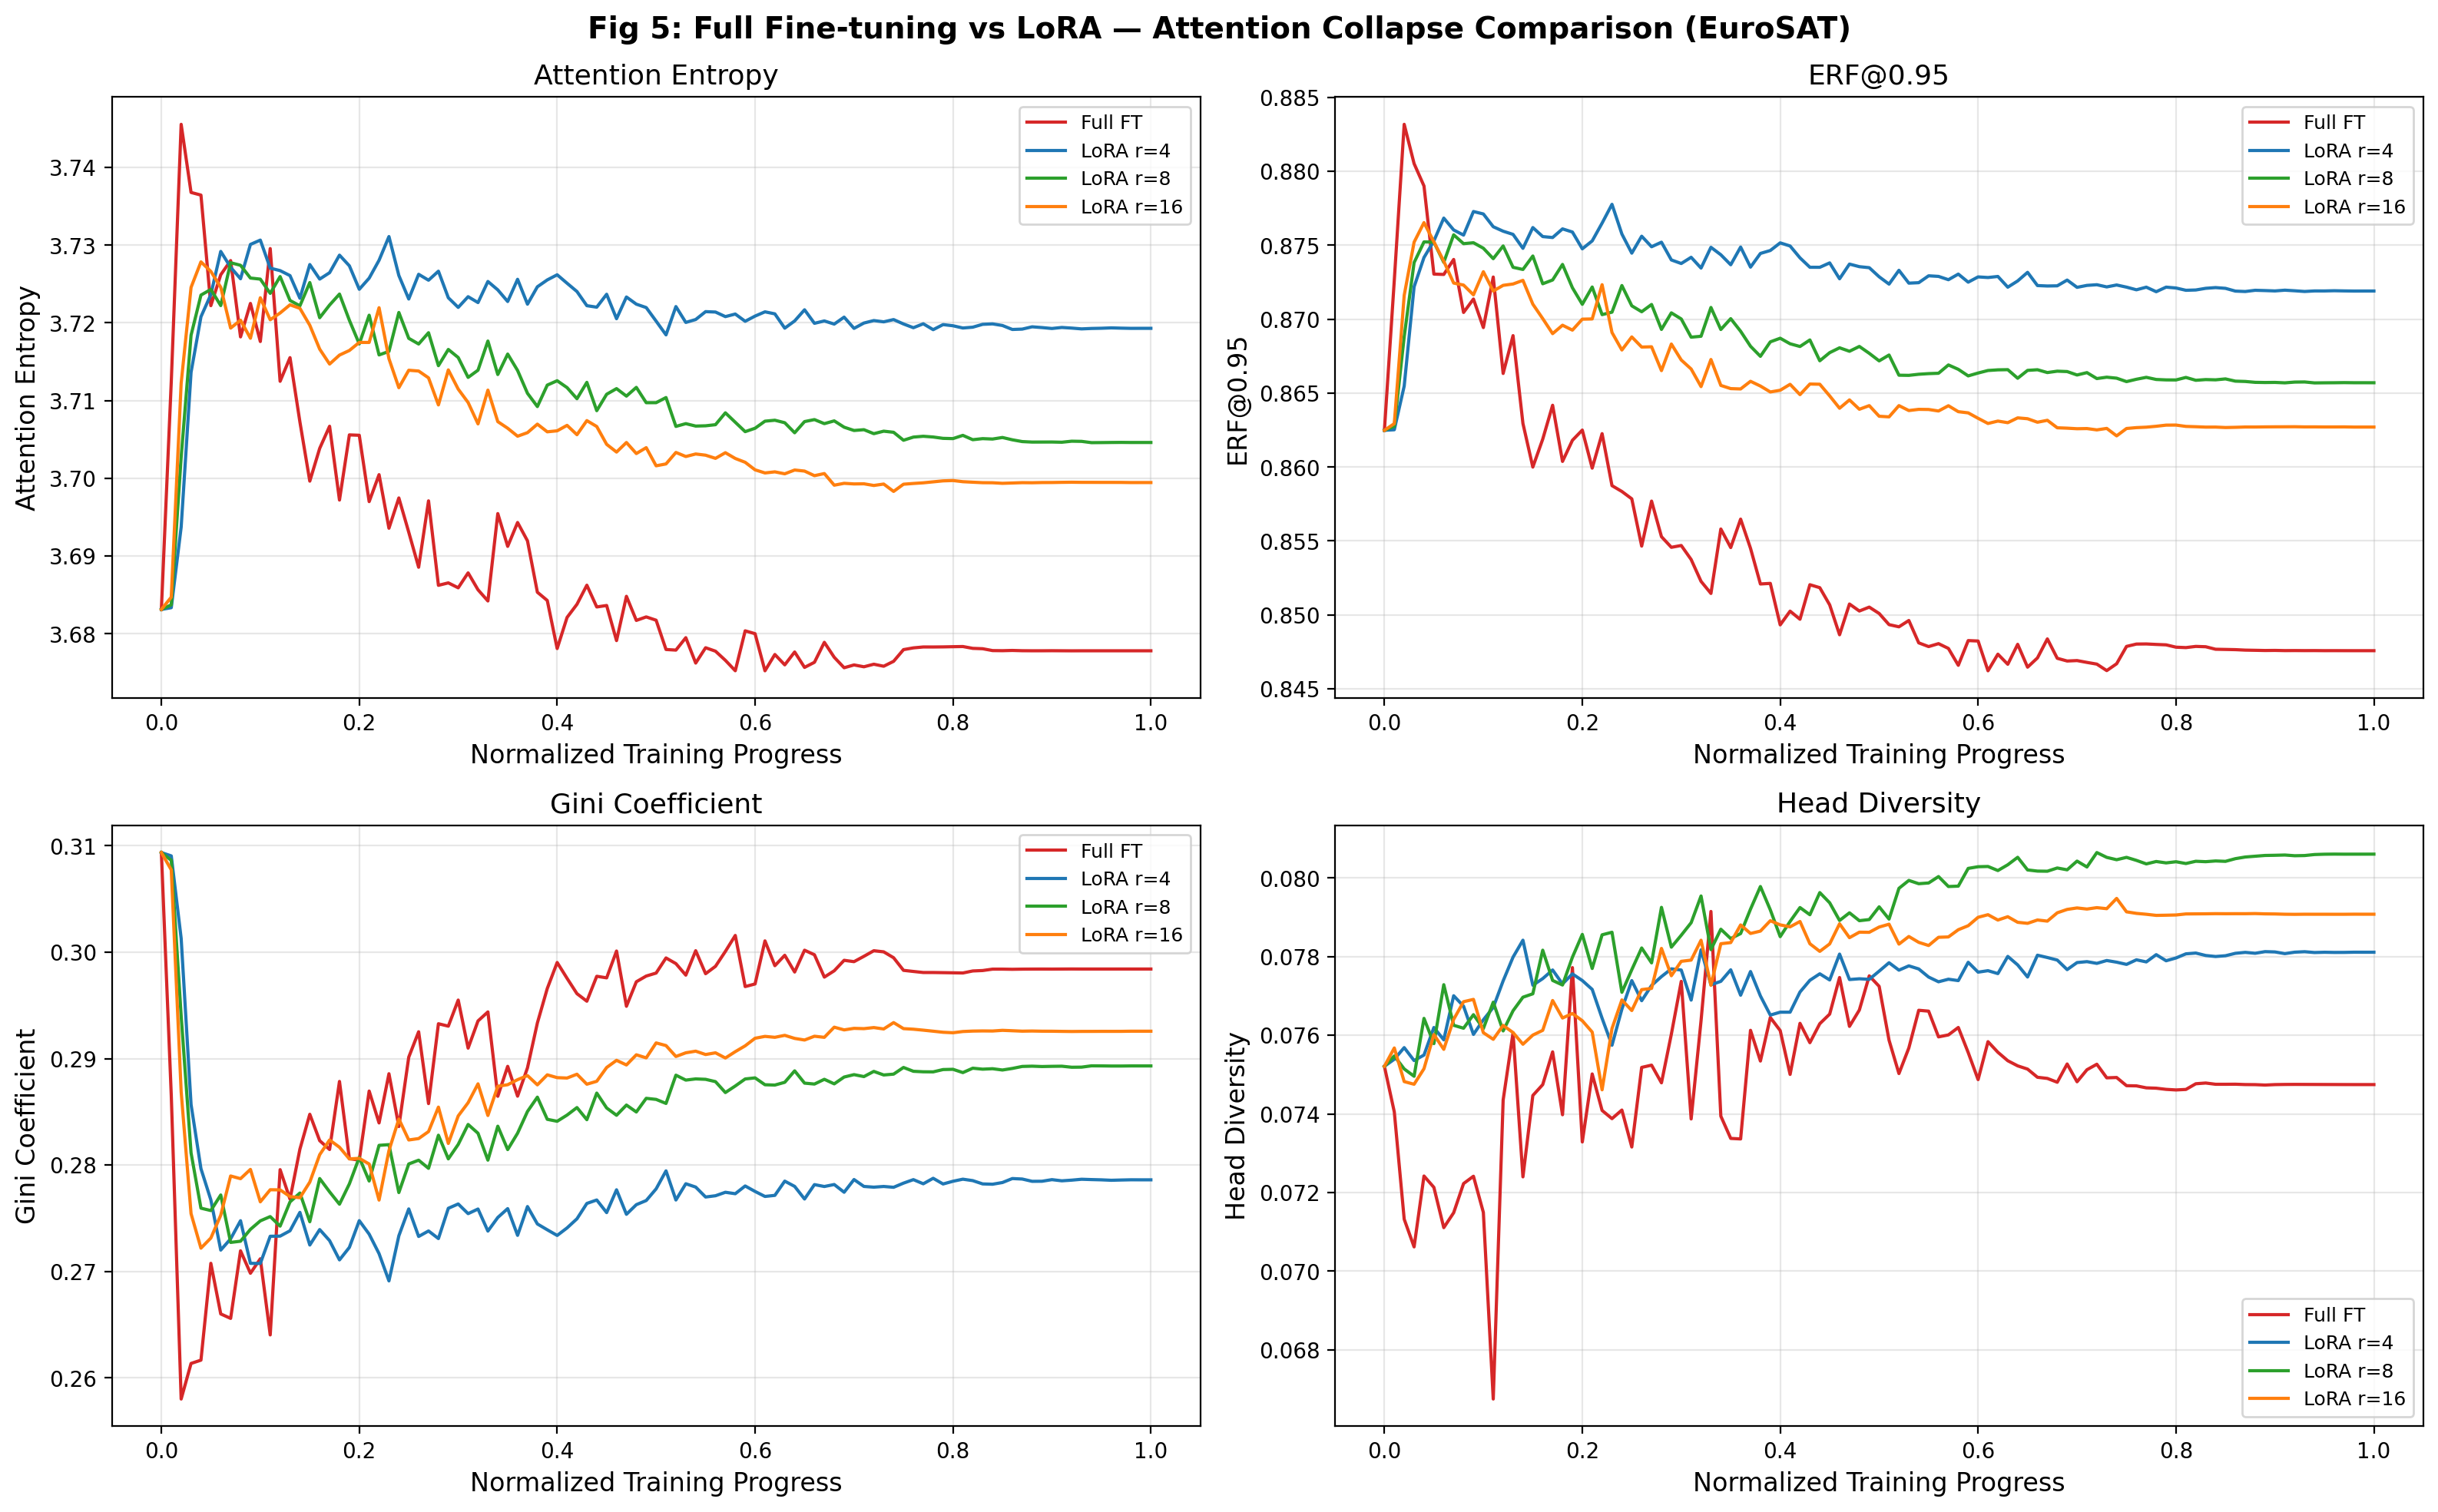
\includegraphics[width=\textwidth]{figures/fig5_fullft_vs_lora.png}
\caption{EuroSAT full fine-tuning versus LoRA. LoRA increases entropy and ERF relative to the pretrained baseline, whereas full fine-tuning remains near neutral to mildly contractive.}\label{fig:ft-vs-lora}
\end{figure}

\subsection{Statistical Evidence and Layerwise Patterns}
Figure~\ref{fig:layer-heatmap} shows that the direction and magnitude of per-layer entropy change depend on both dataset and adaptation regime. However, because layers within a single trained model are not statistically independent, we do not treat these per-layer comparisons as formal evidence of independence. Instead, we interpret the layerwise patterns descriptively and reserve inferential claims for analyses whose sampling assumptions are more defensible.

\begin{table}[t]
\centering
\caption{Corrected inferential statistics. Exact permutation tests are used for the five-point learning-rate analysis. Holm--Bonferroni correction is applied across the regularizer family; no regularizer configuration survives this correction.}
\label{tab:stats}
\small
\resizebox{\columnwidth}{!}{%
\begin{tabular}{llrrl}
\toprule
Comparison & Test & Statistic & $p$-value & Note \\
\midrule
LR vs. $\Delta$Entropy & Exact permutation Pearson $r$ & -0.893 & 0.0333 & $n=5$ learning rates \\ 
LR vs. $\Delta$Entropy & Exact permutation Spearman $\rho$ & -1.000 & 0.0167 & Small-$n$ exact test \\ 
APR $\lambda=0.01$ vs. baseline & Paired per-layer t-test & 2.132 & 0.2194 & Holm--Bonferroni adjusted \\ 
Entropy floor $\lambda=0.1$ vs. baseline & Paired per-layer t-test & 2.638 & 0.1154 & No regularizer survives Holm correction \\ 
\bottomrule
\end{tabular}
}
\end{table}


The clearest corrected inferential result concerns the learning rate. When the five EuroSAT full fine-tuning learning rates are analyzed with exact permutation tests, the negative association between learning rate and $\Delta$entropy remains significant (Pearson $p = 0.0333$; Spearman $p = 0.0167$). By contrast, the regularization family no longer contains a configuration that survives Holm--Bonferroni correction, including entropy floor with $\lambda = 0.1$.

\begin{figure}[H]
\centering
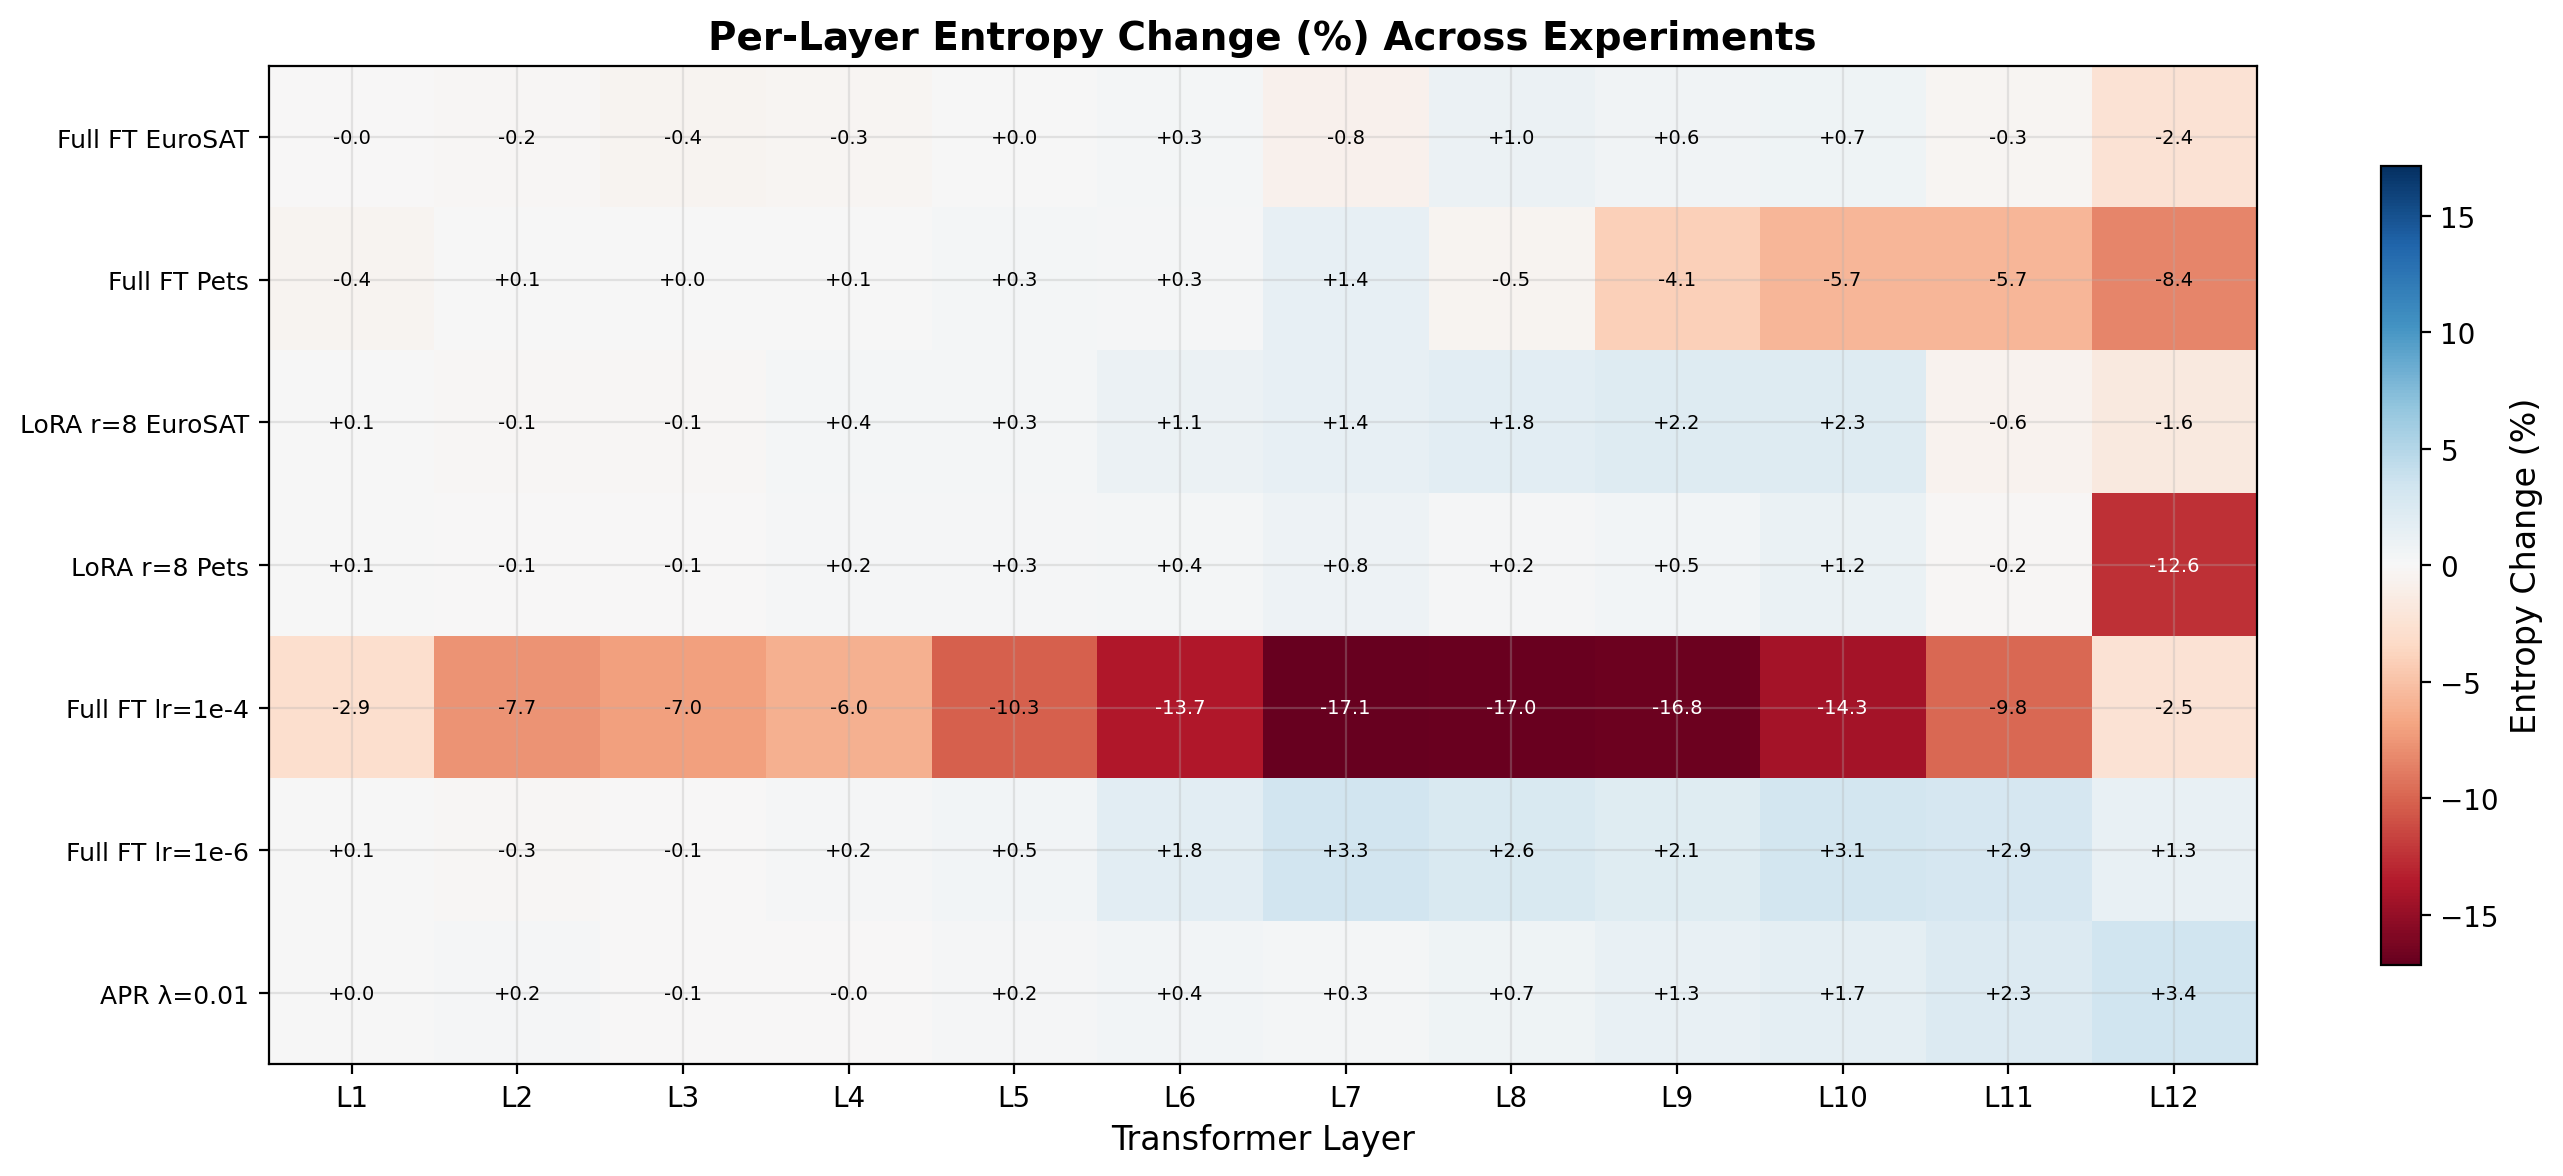
\includegraphics[width=\textwidth]{figures/fig10_per_layer_delta_heatmap.png}
\caption{Per-layer entropy change across selected experiments. The sign and magnitude of the change depend on the training regime and the dataset.}\label{fig:layer-heatmap}
\end{figure}

\begin{figure}[H]
\centering
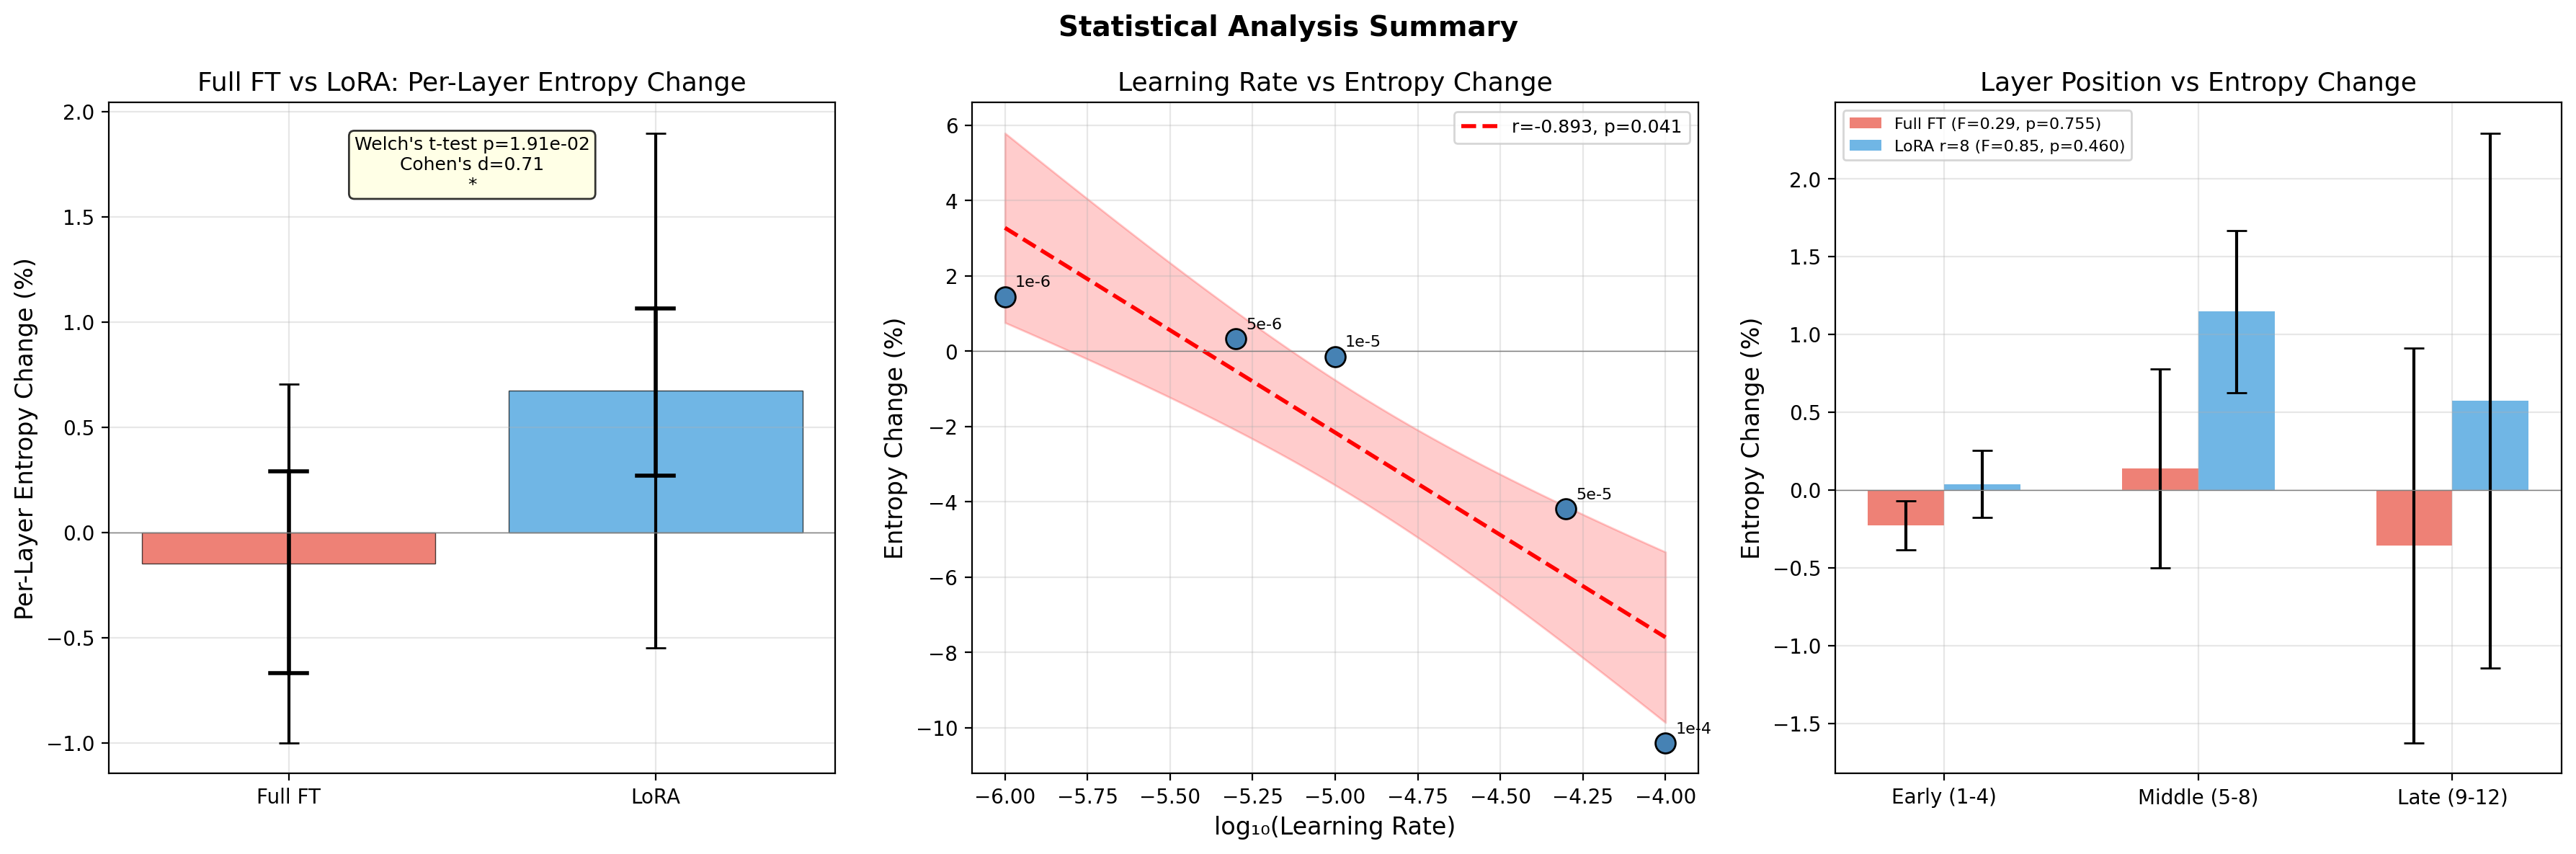
\includegraphics[width=\textwidth]{figures/fig11_statistical_summary.png}
\caption{Summary of exploratory per-layer comparisons and corrected statistical analyses, including the learning-rate trend and layer-group summaries.}\label{fig:stats-summary}
\end{figure}

\subsection{Impact of Learning Rate on Structural Dynamics}
Among the manipulated hyperparameters, the learning rate appeared to be the dominant control variable for structural change. Table~\ref{tab:lr-sweep} shows a monotonic trend: entropy increases at $10^{-6}$, is nearly neutral at $10^{-5}$, and decreases sharply at $5 \times 10^{-5}$ and $10^{-4}$. Under exact permutation testing on the five learning-rate settings, the Pearson correlation between $\log_{10}(\mathrm{LR})$ and $\Delta$entropy is $-0.893$ ($p = 0.0333$), while the Spearman coefficient is $-1.0$ ($p = 0.0167$).

\begin{table}[t]
\centering
\caption{Learning-rate sweep for EuroSAT full fine-tuning. Entropy decreases monotonically as the learning rate increases across the tested range.}
\label{tab:lr-sweep}
\small
\resizebox{\columnwidth}{!}{%
\begin{tabular}{lrrrrrr}
\toprule
LR & Task Acc. (\%) & $\Delta$Entropy (\%) & $\Delta$ERF (\%) & $\Delta$Gini (\%) & CIFAR-100 ZS (\%) & Flowers102 ZS (\%) \\
\midrule
1e-6 & 98.85 & +1.45 & +1.94 & -16.60 & --- & --- \\
5e-6 & 99.11 & +0.33 & -0.49 & -6.68 & --- & --- \\
1e-5 & 99.30 & -0.14 & -1.73 & -3.54 & 12.71 & 1.37 \\
5e-5 & 98.89 & -4.19 & -8.48 & +23.44 & 2.07 & 0.88 \\
1e-4 & 97.85 & -10.40 & -18.02 & +56.94 & 1.86 & 0.98 \\
\bottomrule
\end{tabular}
}
\end{table}


\begin{figure}[H]
\centering
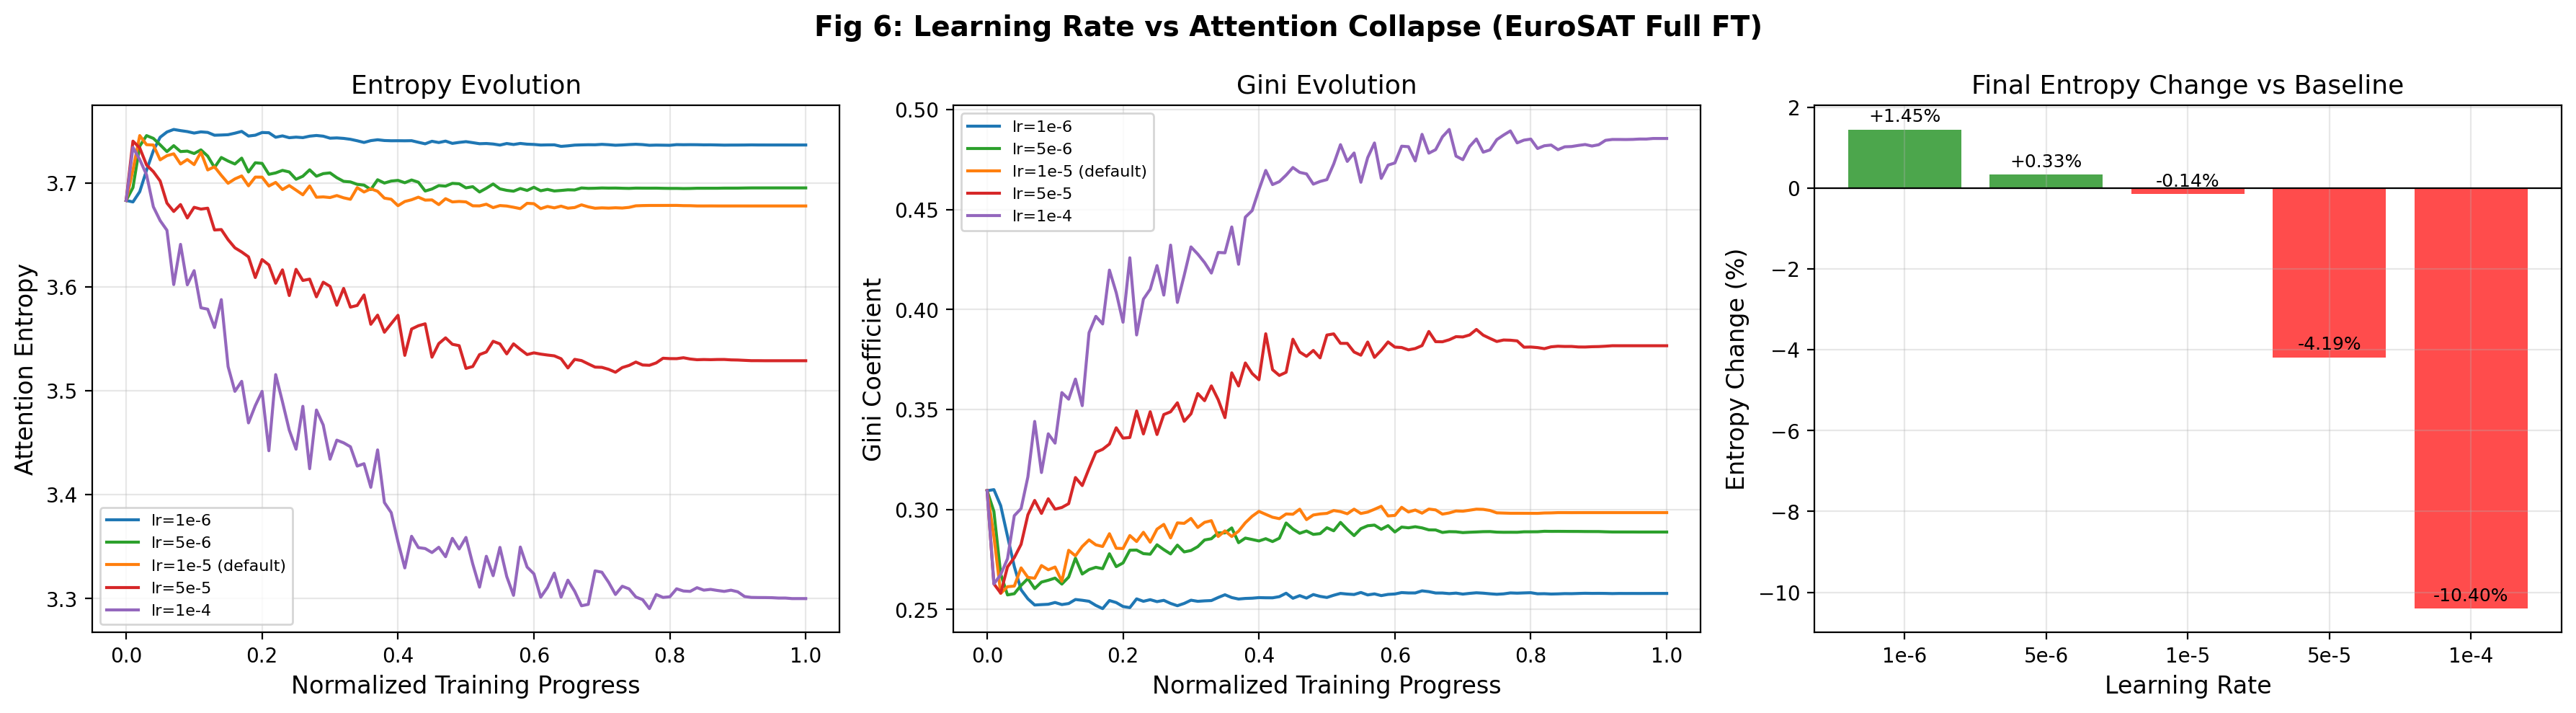
\includegraphics[width=\textwidth]{figures/fig6_lr_sweep.png}
\caption{Learning-rate sweep for EuroSAT full fine-tuning. Larger learning rates produce stronger entropy decreases and stronger ERF contraction.}\label{fig:lr-sweep}
\end{figure}

This result matters because it reframes collapse as an optimization-scale phenomenon rather than merely a binary property of full fine-tuning versus parameter-efficient tuning. In the revised analysis, the effect remains when the small-sample correlation test is recomputed exactly rather than through asymptotic approximations.

\subsection{Regularization and Training Dynamics}
Table~\ref{tab:regularization} summarizes the regularization study. Both APR and entropy-floor regularization shift entropy upward relative to the no-regularizer baseline, while preserving high task accuracy. However, after Holm--Bonferroni correction across the regularizer family, no individual configuration remains statistically significant within the exploratory per-layer comparison framework used here. The regularization results should therefore be interpreted as promising but preliminary.

\begin{table}[t]
\centering
\caption{Regularization study on EuroSAT full fine-tuning. Among individually tested regularizers, entropy floor with $\lambda=0.1$ is the only setting with a paired per-layer entropy difference reaching $p<0.05$ in the current analysis.}
\label{tab:regularization}
\small
\resizebox{\columnwidth}{!}{%
\begin{tabular}{lrrrr}
\toprule
Setting & Task Acc. (\%) & $\Delta$Entropy (\%) & $\Delta$ERF (\%) & $\Delta$Gini (\%) \\
\midrule
No regularizer & 99.30 & -0.14 & -1.73 & -3.54 \\
APR $\lambda=0.01$ & 99.26 & +0.86 & +1.50 & -8.83 \\
APR $\lambda=0.1$ & 99.19 & +0.56 & +1.03 & -5.36 \\
APR $\lambda=1.0$ & 98.96 & +0.09 & +0.16 & -0.75 \\
Entropy floor $\lambda=0.01$ & 99.11 & +0.58 & -0.09 & -6.41 \\
Entropy floor $\lambda=0.1$ & 99.07 & +0.79 & +0.30 & -8.22 \\
Weight decay 0.0 & 99.19 & -0.18 & -1.81 & -3.16 \\
Weight decay 0.1 & 99.15 & -0.25 & -1.90 & -2.38 \\
\bottomrule
\end{tabular}
}
\end{table}


\begin{figure}[H]
\centering
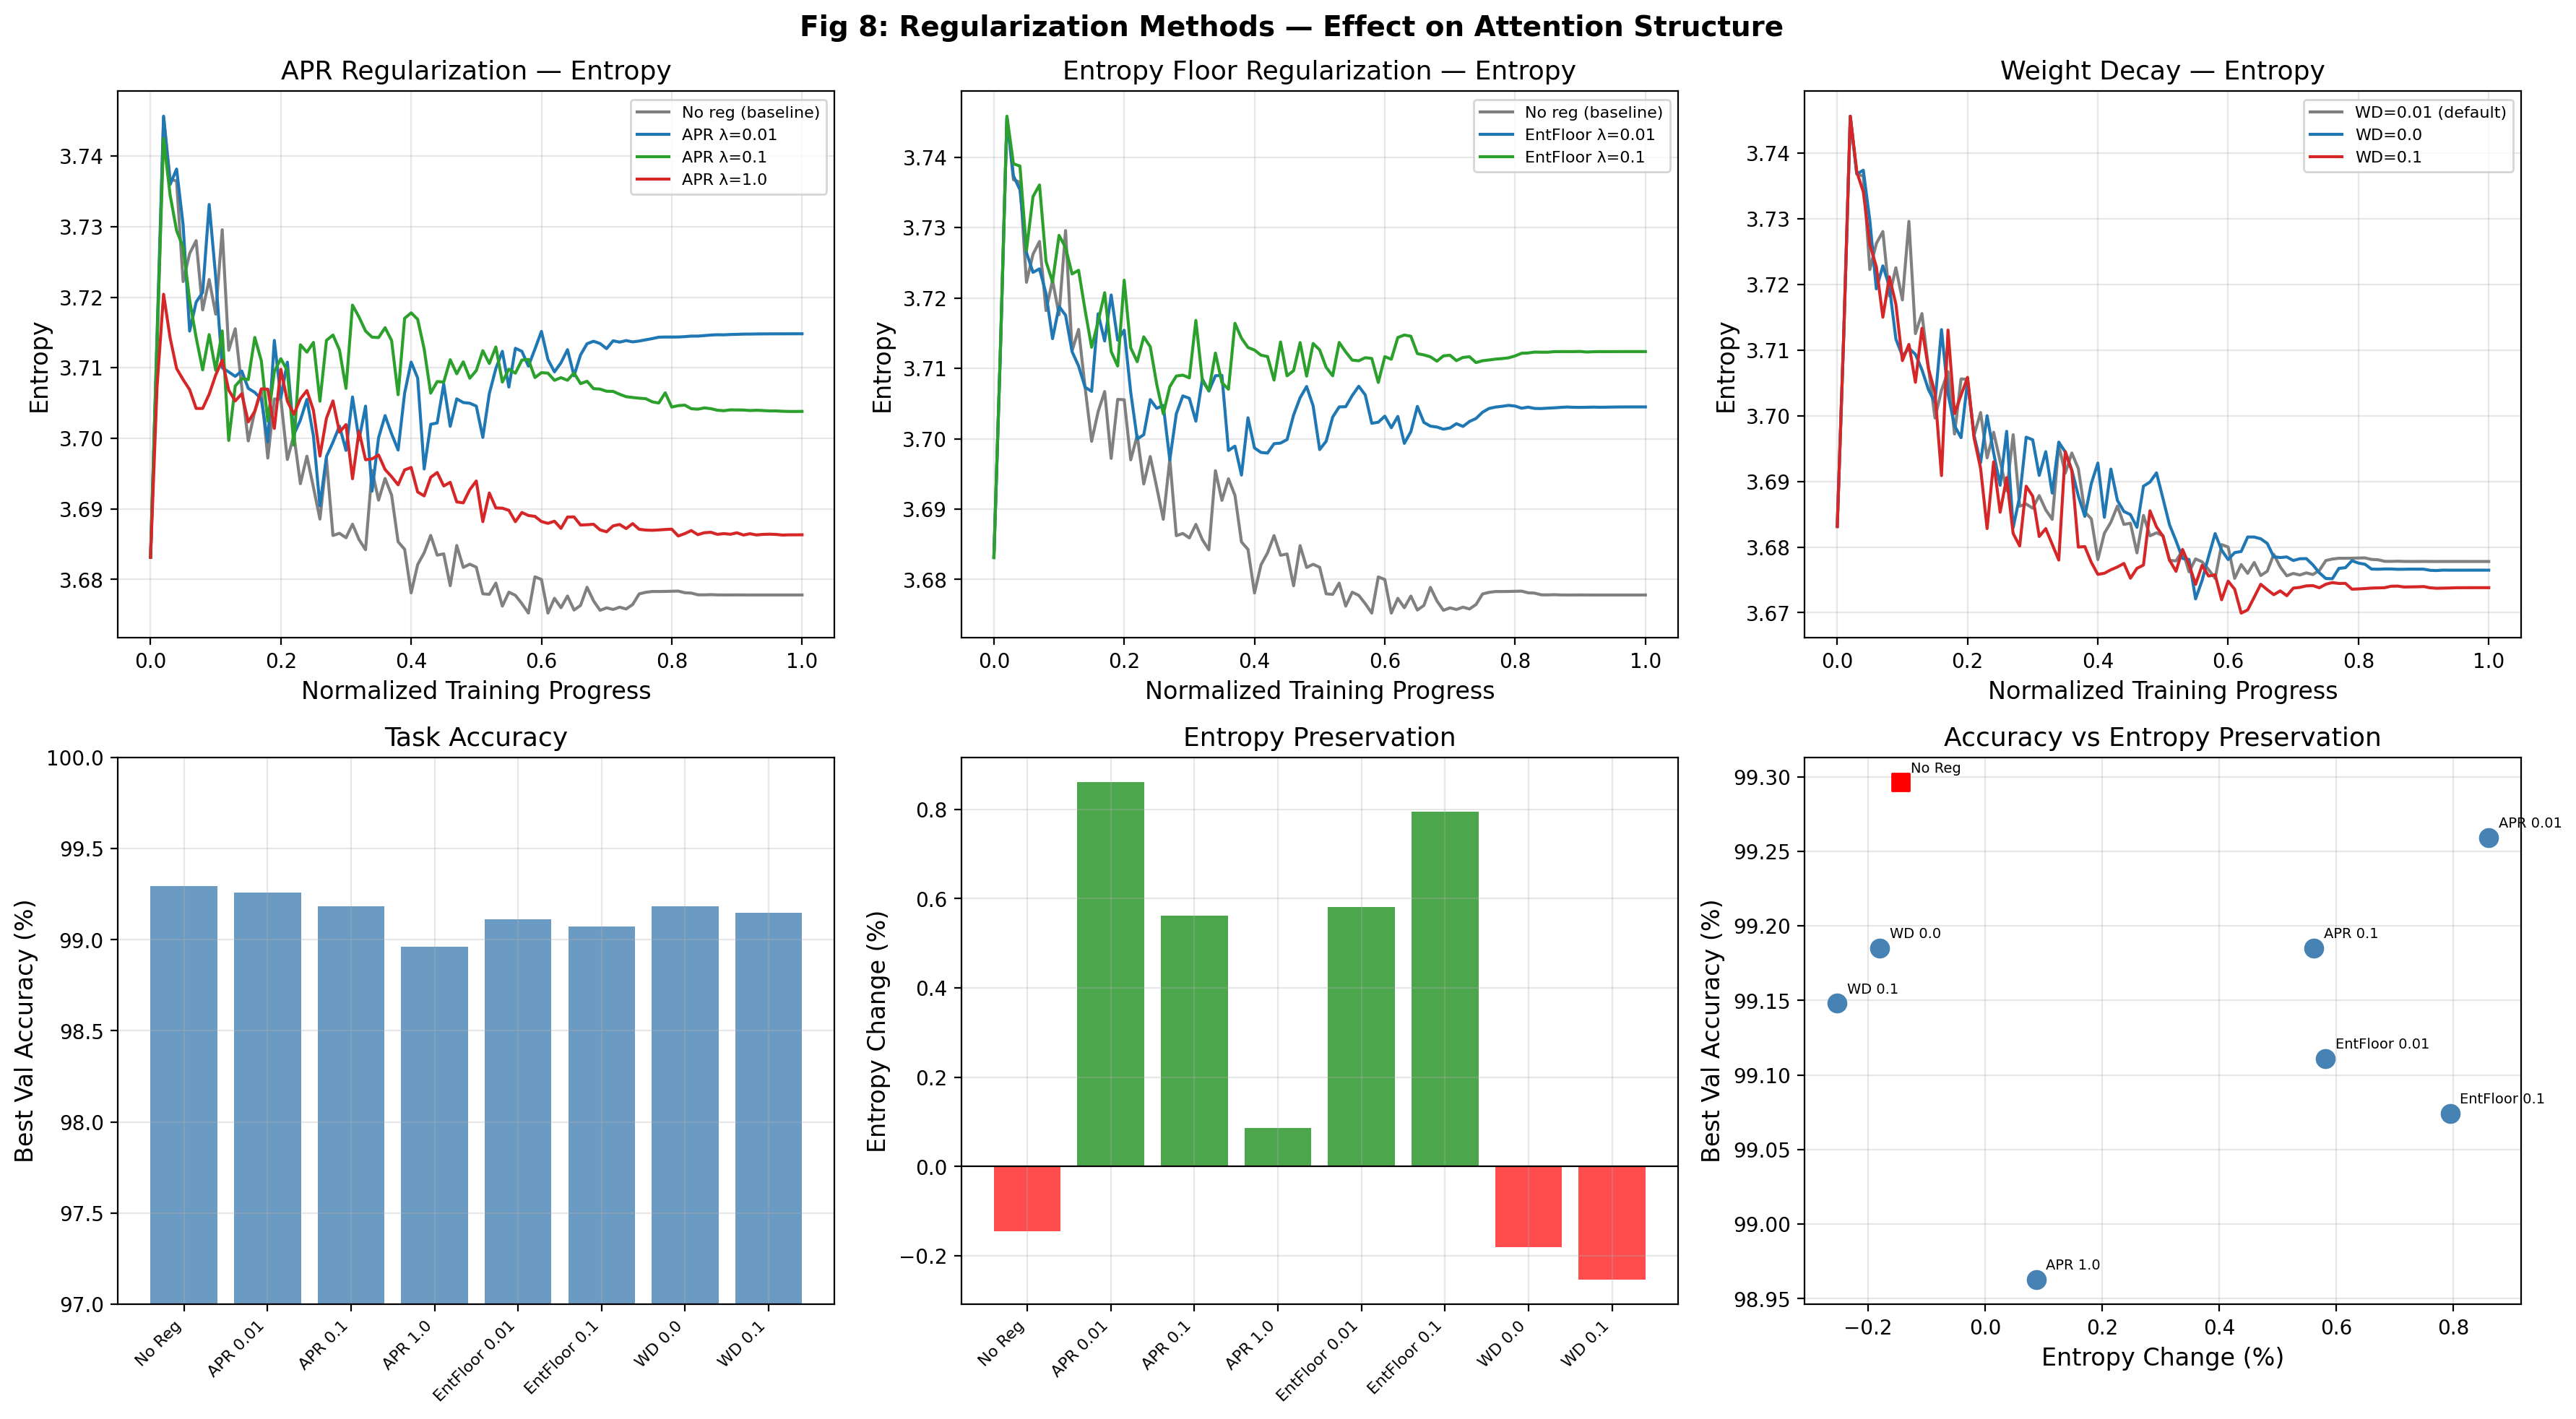
\includegraphics[width=\textwidth]{figures/fig8_regularization.png}
\caption{Regularization results. Both APR and entropy floor preserve a broader attention structure than the no-regularizer baseline in descriptive terms. Still, none of the tested settings survives Holm--Bonferroni correction across the regularizer family.}\label{fig:regularization}
\end{figure}

Figure~\ref{fig:dynamics} complements the final-state tables by showing training trajectories and collapse-onset markers. The main qualitative lesson is that structural drift appears early when the learning rate is high, whereas LoRA traces a flatter path. Again, this constitutes observational evidence rather than a mechanistic proof.

\begin{figure}[H]
\centering
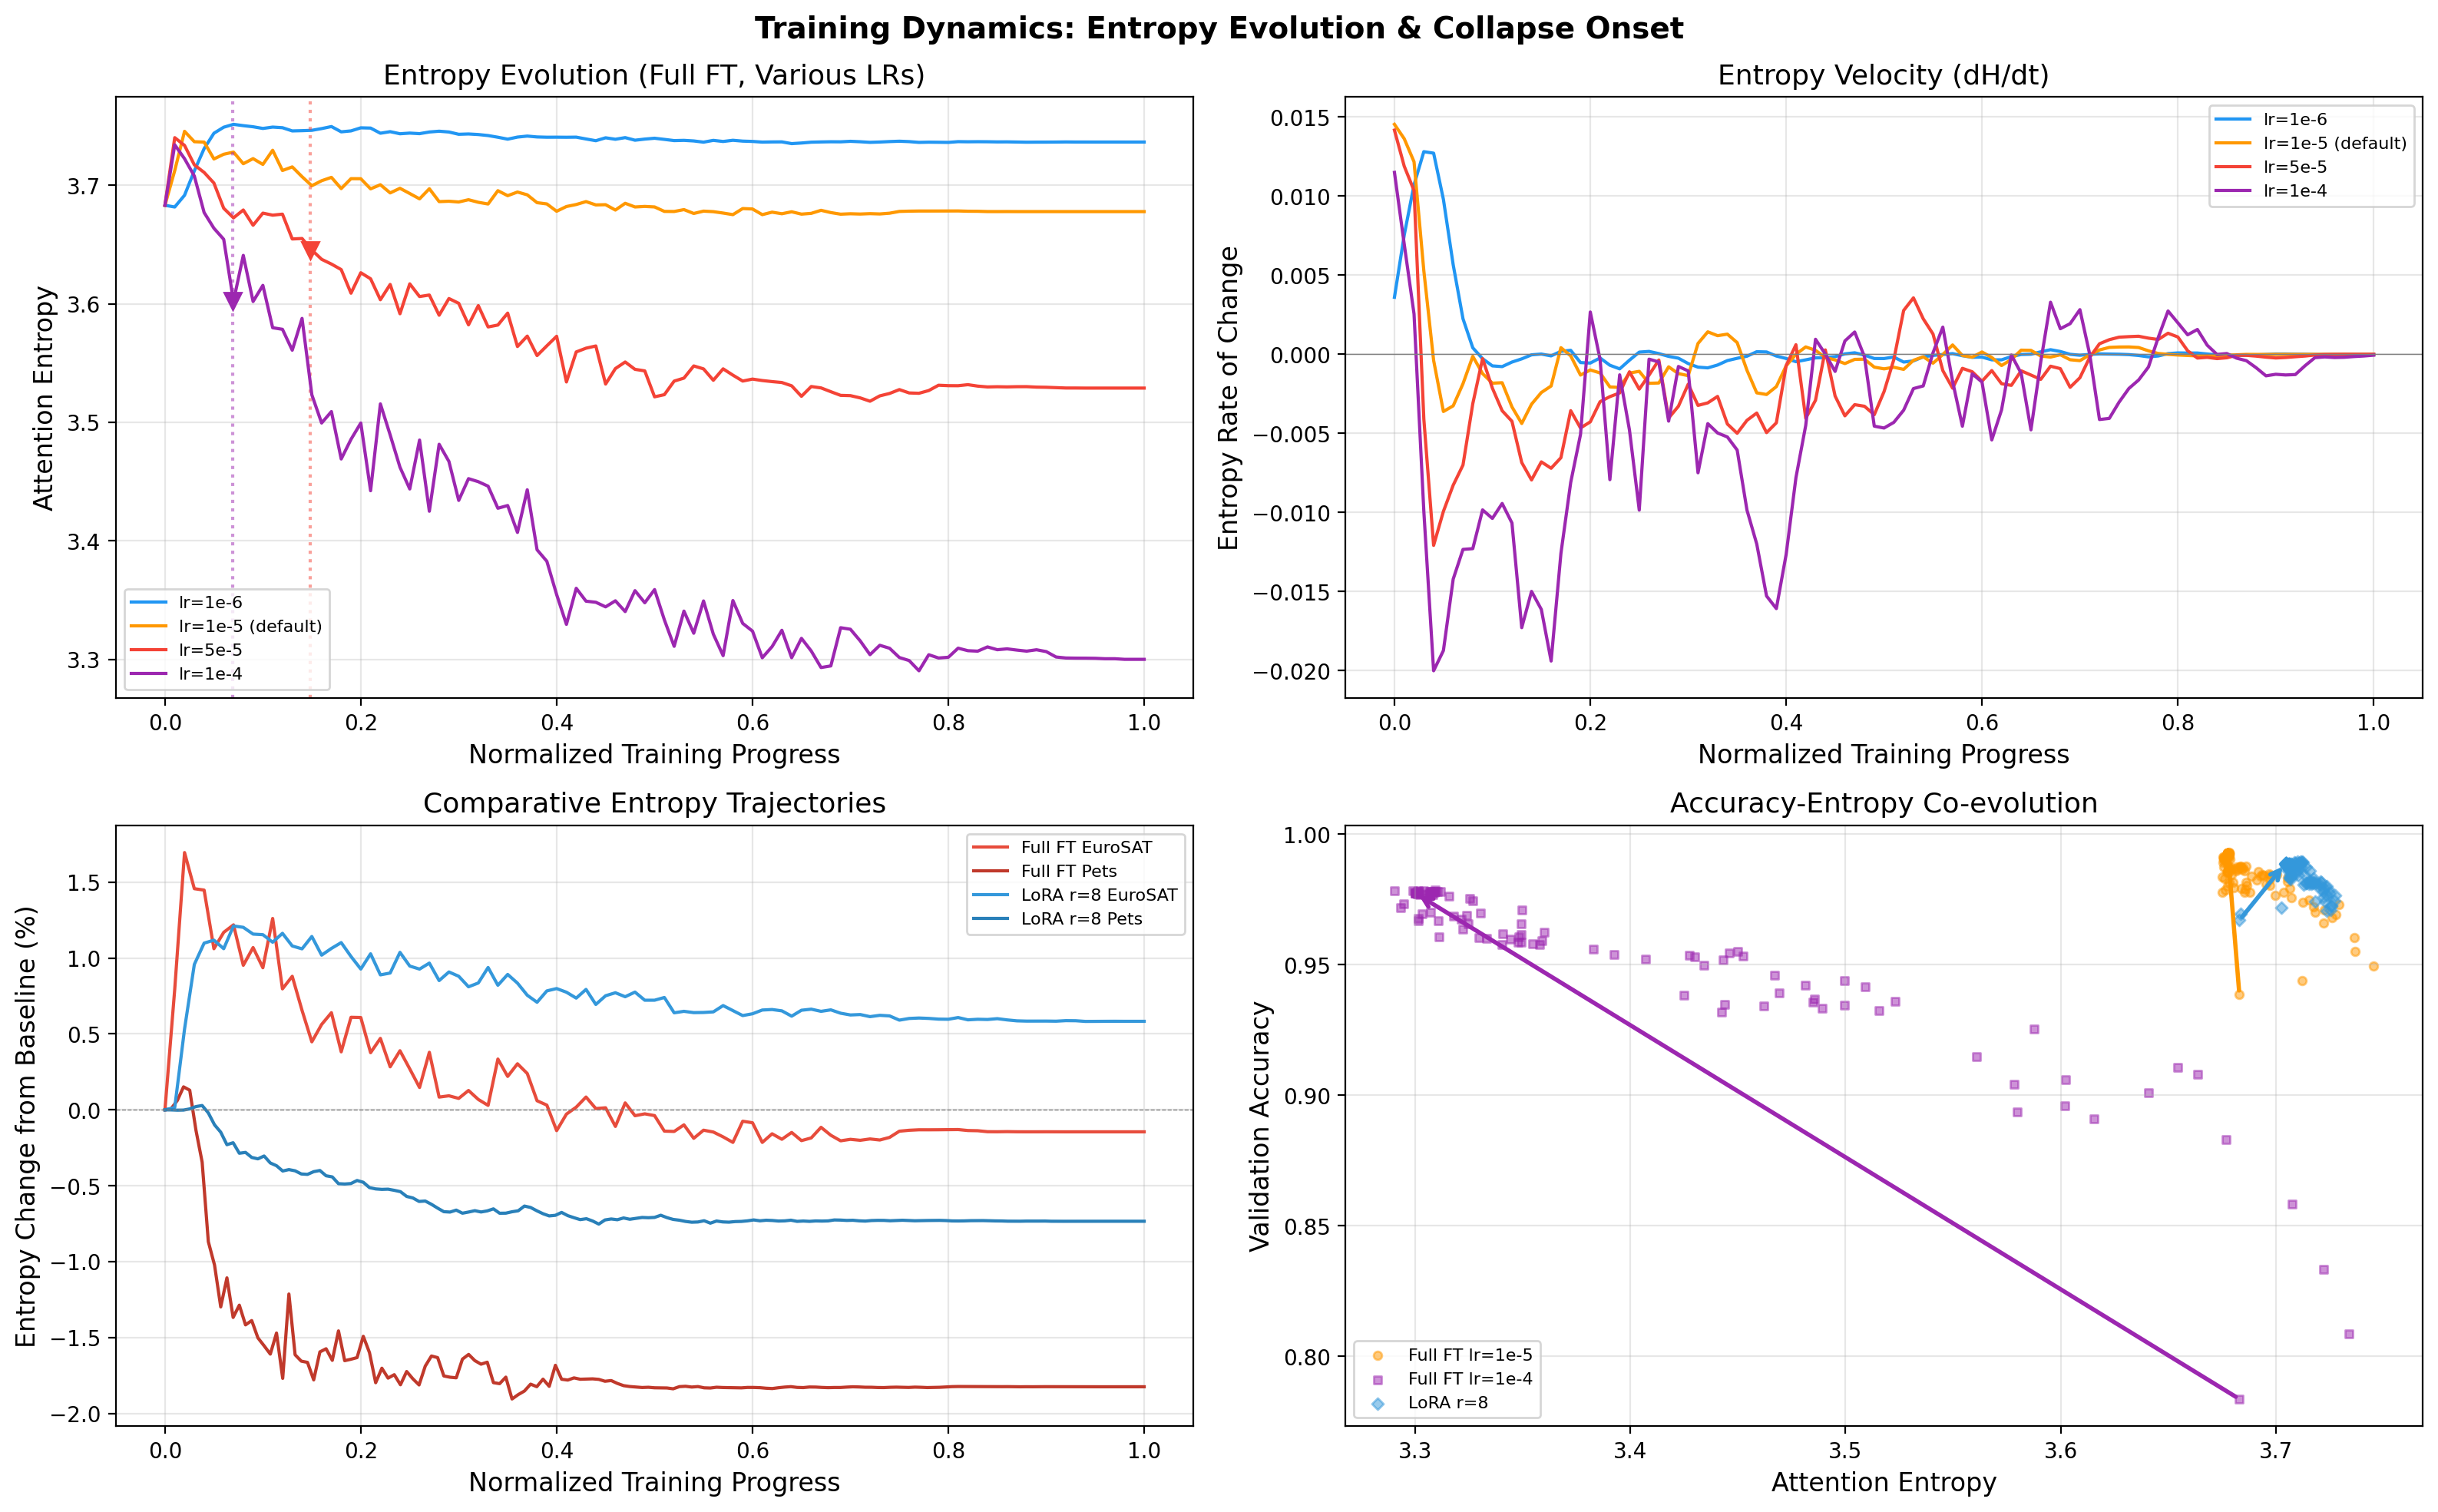
\includegraphics[width=\textwidth]{figures/fig12_training_dynamics.png}
\caption{Training dynamics and collapse-onset analysis. High-learning-rate full fine-tuning exhibits the earliest and strongest decrease in entropy.}\label{fig:dynamics}
\end{figure}

\subsection{Auxiliary Structural Validation}
To test whether the main conclusions are specific to CLS-to-patch entropy, Table~\ref{tab:auxiliary-validation} reports supplementary rollout, patch-to-patch, representational-similarity, and subset-sensitivity analyses for the clearest EuroSAT comparison. LoRA $r = 8$ exhibits higher rollout entropy, larger rollout ERF@0.95, lower rollout Gini, and higher patch-to-patch entropy than full fine-tuning, indicating that the broader-support pattern is not confined to the original CLS-to-patch metric. LoRA also yields a higher mean layerwise centered kernel alignment to the pretrained model (0.815 versus 0.694), suggesting less representational drift. Finally, the coefficient of variation of the entropy metric across five balanced evaluation subsets is below 0.001 for both methods, indicating that the reported structural metrics are not highly sensitive to the choice of evaluation images.

\begin{table}[t]
\centering
\caption{Auxiliary validation analyses beyond CLS-to-patch entropy. Rollout and patch-to-patch metrics indicate broader attention support for LoRA than for Full FT on EuroSAT, while layerwise CKA shows higher representational similarity to the pretrained encoder. The subset-sensitivity coefficient of variation (CV) is low for both methods, indicating that the reported metrics are stable across five balanced evaluation subsets.}
\label{tab:auxiliary-validation}
\begin{adjustwidth}{-\extralength}{0cm}
\small
\begin{tabularx}{\fulllength}{LCCCCCCC}
\toprule
Model & Rollout Entropy & Rollout ERF@0.95 & Rollout Gini & PTP Entropy & Mean CKA & Entropy CV \\
\midrule
Full FT EuroSAT & 5.593 & 0.944 & 0.090 & 4.721 & 0.694 & 0.0006 \\
\addlinespace[4.5pt]
LoRA $r=8$ EuroSAT & 5.605 & 0.952 & 0.064 & 4.794 & 0.815 & 0.0005 \\
\bottomrule
\end{tabularx}
\end{adjustwidth}
\end{table}


\subsection{Zero-Shot Transfer: Evidence and Caveats}
The zero-shot table is included for completeness, but its interpretation requires care. Reliable evaluation of LoRA models requires an inference procedure that activates the learned adapters in the image encoder. Accordingly, the EuroSAT LoRA models were reevaluated using this procedure, while the pretrained baseline was retained from the standard CLIP evaluation pipeline.

\begin{table}[t]
\centering
\caption{Zero-shot transfer accuracy (\%) on CIFAR-100 and Flowers102 after EuroSAT fine-tuning. LoRA preserves substantially more CIFAR-100 accuracy than full fine-tuning, while Flowers102 values are uniformly low for all models and should be treated as supplemental evidence only.}
\label{tab:zeroshot}
\small
\resizebox{0.8\columnwidth}{!}{%
\begin{tabular}{lrr}
\toprule
Model & CIFAR-100 (\%) & Flowers102 (\%) \\
\midrule
Pretrained & 60.22 & 0.20 \\
Full FT (EuroSAT) & 9.43 & 1.37 \\
LoRA $r=4$ (EuroSAT) & 40.51 & 1.27 \\
LoRA $r=8$ (EuroSAT) & 47.28 & 0.78 \\
LoRA $r=16$ (EuroSAT) & 39.35 & 0.98 \\
\bottomrule
\end{tabular}
}
\end{table}


The revised results materially change the interpretation. LoRA does not preserve the full pretrained CIFAR-100 accuracy of 60.22\%, but it degrades far less than full fine-tuning: LoRA $r = 8$ reaches 47.28\%, compared with 9.43\% for full fine-tuning. LoRA, therefore, remains structurally and functionally more conservative than full fine-tuning in this setting. Still, the earlier, stronger claim of near-perfect transfer preservation is not supported once adapters are evaluated correctly.

The Flowers102 values are also uniformly low (all below 1.37\%), suggesting that the current prompt and label specification do not provide a sufficiently reliable primary benchmark for this study. For that reason, Flowers102 is treated as supplemental rather than central evidence.

\begin{figure}[H]
\centering
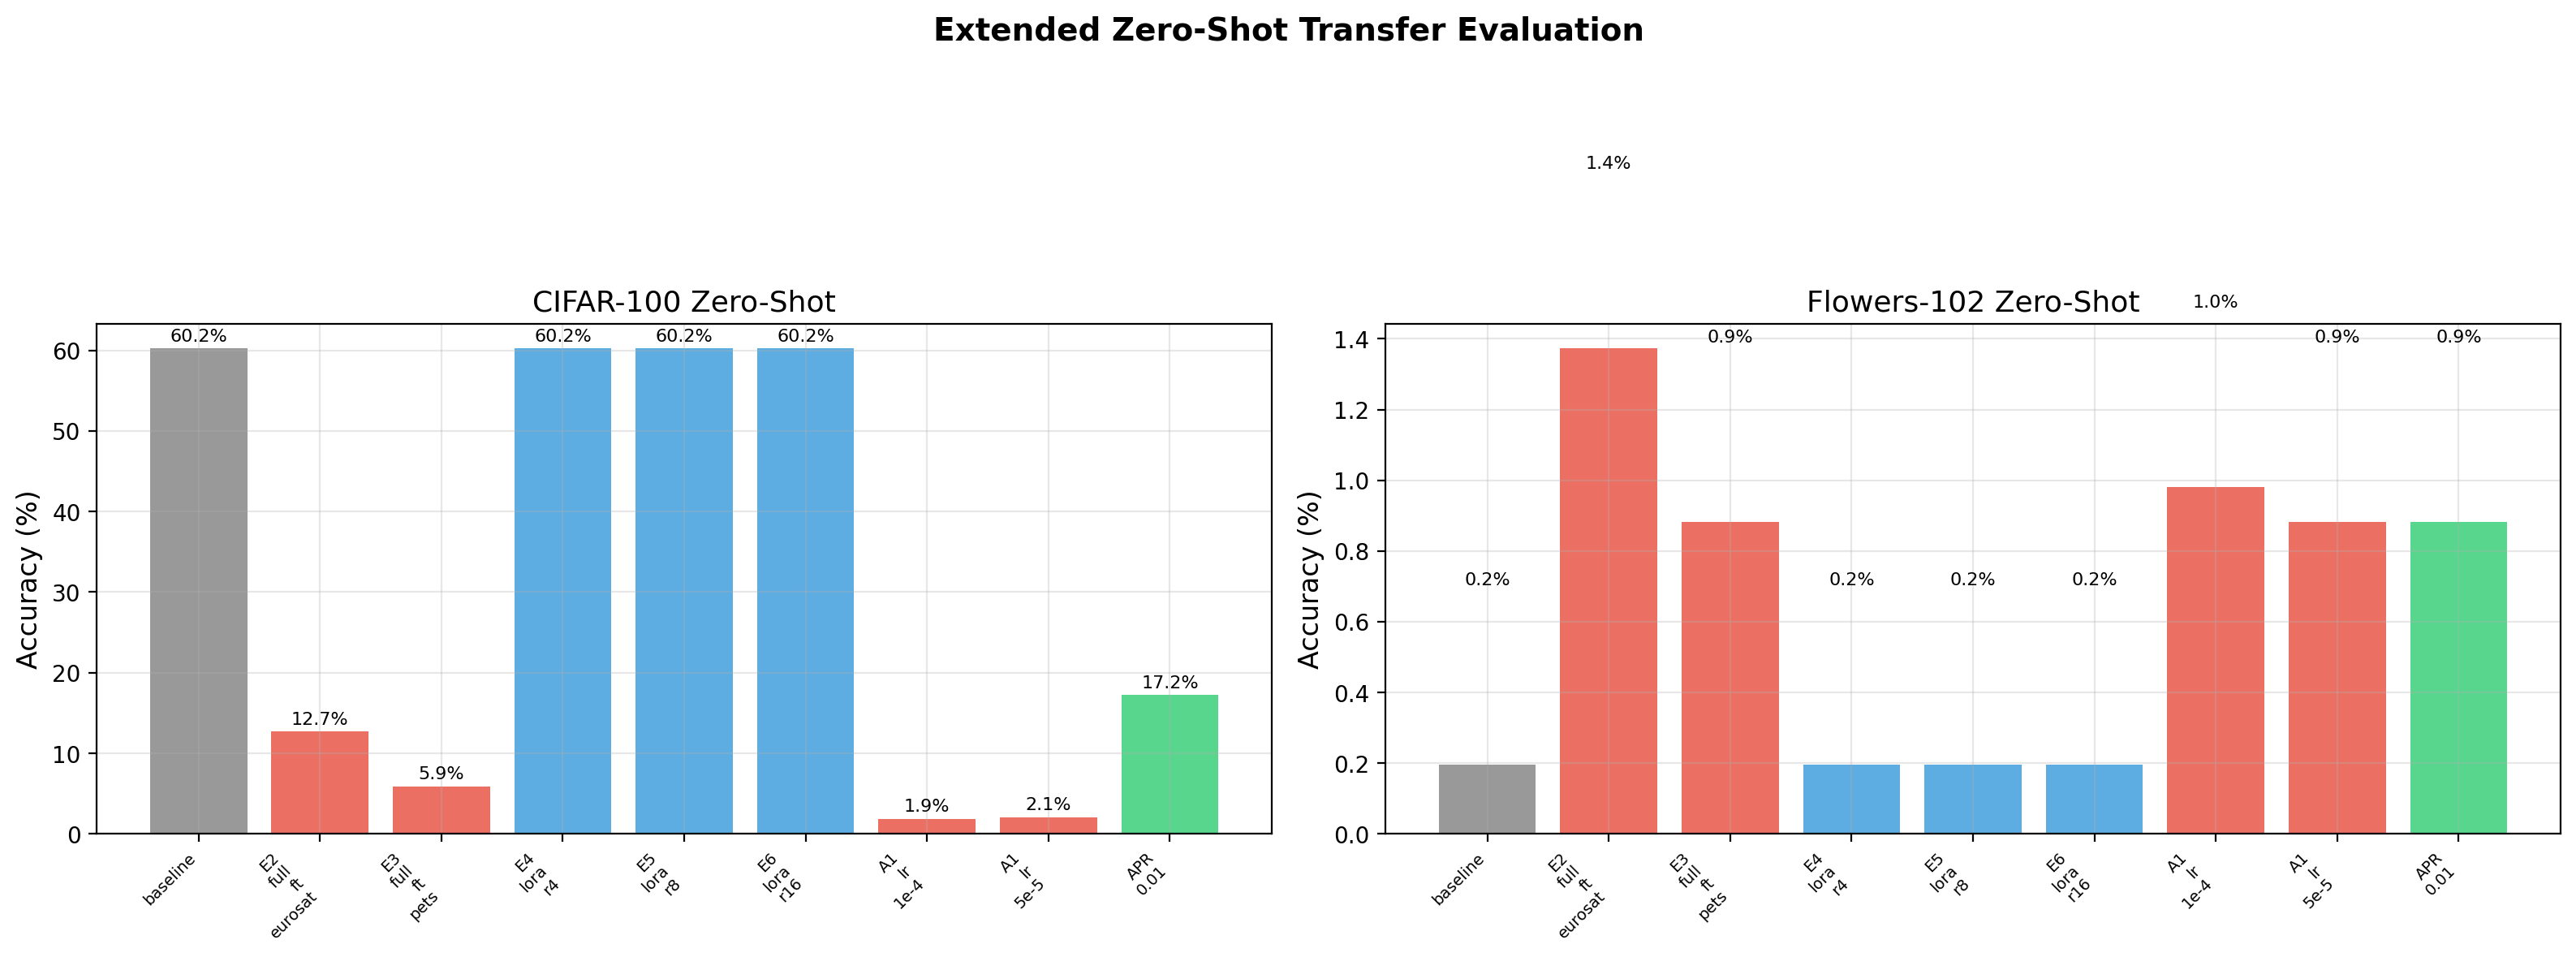
\includegraphics[width=\textwidth]{figures/fig15_zeroshot_extended.png}
\caption{Extended zero-shot evaluation under the study's evaluation protocol. CIFAR-100 is the more interpretable benchmark, whereas the Flowers102 values are uniformly too low to support strong conclusions.}\label{fig:zeroshot}
\end{figure}

\section{Discussion}
The results suggest that attention structural change is neither negligible nor uniform across adaptation strategies. Across the experiments analyzed here, full fine-tuning tends to narrow attention support, particularly on Oxford-IIIT Pets. In contrast, EuroSAT LoRA maintains or slightly broadens attention support relative to the pretrained baseline. The auxiliary rollout and patch-to-patch analyses reinforce this interpretation, and the centered kernel alignment results indicate that LoRA remains closer to the pretrained representation geometry than full fine-tuning.

The learning-rate sweep further indicates that the magnitude of optimization steps is a key determinant of structural change. This observation is noteworthy because it implies that attention contraction is not simply an intrinsic property of full fine-tuning; rather, it is strongly modulated by training scale. From a practical perspective, this suggests that structurally conservative adaptation may be achievable not only through parameter-efficient methods such as LoRA but also through careful optimization control.

The regularization results provide only cautious support for this interpretation. Although APR and entropy-floor regularization shift the model toward broader attention distributions, the available per-layer evidence does not survive a family-wise multiple-comparison correction. These results, therefore, motivate but do not yet establish regularization as a reliable solution.

\section{Conclusions}
This study examined structural changes in attention during fine-tuning of CLIP through a comparative analysis of full fine-tuning, LoRA, and regularized adaptation. The analysis combines exact tests, where appropriate, with supplementary rollout, patch-to-patch, centered-kernel alignment, and subset-sensitivity measurements to triangulate the main findings. Under this deliberately conservative inferential framing, the central qualitative conclusion remains intact: adaptation regime and learning rate materially affect attention structure, and LoRA is substantially less disruptive than full fine-tuning on the clearest EuroSAT comparison. At the same time, the study delineates what remains unresolved, particularly regarding run-level inference and the generality of the findings across seeds, backbones, and transfer benchmarks.

\authorcontributions{R.X. conceived the study, designed and conducted all experiments, performed the statistical analyses, and wrote the manuscript. The author has read and agreed to the published version of the manuscript.}

\funding{This research received no external funding.}

\institutionalreview{Not applicable.}

\informedconsent{Not applicable.}

\dataavailability{The code, manuscript source, figures, tables, and analysis artifacts supporting this study are publicly available at \url{https://github.com/xiaruize0911/Attention_Collapse_in_CLIP_Fine-tuning_repo}. Additional derived outputs used in this study are available from the corresponding author on reasonable request.}

\acknowledgments{The author thanks the open-source software and dataset communities whose tools and benchmarks enabled this study. Computational resources for the experiments were provided through rented NVIDIA A40 instances on RunPod.}

\conflictsofinterest{The author declares no conflicts of interest.}

\abbreviations{Abbreviations}{
\noindent
\begin{tabular}{@{}ll}
APR & Attention preservation regularization\\
CKA & Centered kernel alignment\\
CLIP & Contrastive Language--Image Pretraining\\
ERF & Effective receptive field\\
FT & Fine-tuning\\
LoRA & Low-rank adaptation
\end{tabular}}

\begin{adjustwidth}{-\extralength}{0cm}
\reftitle{References}
\bibliography{references}
\PublishersNote{}
\end{adjustwidth}

\end{document}
